\documentclass[12pt,a4paper]{article}
\usepackage[utf8]{inputenc}
\usepackage[T1]{fontenc} % For better font encoding and hyphenation
\usepackage[french]{babel}
\usepackage{geometry}
\usepackage{graphicx}
\usepackage{listings}
\usepackage{hyperref} % Should ideally be one of the last packages loaded, but graphicx/xcolor sometimes interact
\usepackage{xcolor}
\usepackage{fancyhdr}
\usepackage{titlesec}
\usepackage{tcolorbox}
\usepackage{enumitem}
\usepackage{booktabs}
\usepackage{array}
\usepackage{longtable}
\usepackage{amsmath}
\usepackage{lmodern} % Use Latin Modern fonts for a slightly crisper look
\usepackage{setspace} % For line spacing
\usepackage[belowskip=5pt,aboveskip=5pt]{caption} % Adjust space around captions

\hypersetup{ % Configuration for hyperref
    colorlinks=true,
    linkcolor=secondaryblue,
    filecolor=magenta,      
    urlcolor=primaryblue,
    citecolor=darkgray,
    pdftitle={Rapport de Projet - Application de Chat Flutter avec BLoC},
    pdfauthor={Youssef Faik},
    pdfsubject={Développement d'une application de chat},
    pdfkeywords={Flutter, BLoC, Chat, Mobile, Application},
    bookmarks=true,
    bookmarksopen=true
}


\setstretch{1.1} % Increase line spacing slightly for readability

\geometry{a4paper, margin=1in, headheight=15pt}

% Color scheme
\definecolor{primaryblue}{RGB}{25, 118, 210}
\definecolor{secondaryblue}{RGB}{63, 81, 181}
\definecolor{lightblue}{RGB}{227, 242, 253}
\definecolor{darkgray}{RGB}{66, 66, 66}
\definecolor{lightgray}{RGB}{245, 245, 245}

% VS Code Dark Theme Colors
\definecolor{vscodeBackground}{RGB}{30, 30, 30}
\definecolor{vscodeText}{RGB}{212, 212, 212}
\definecolor{vscodeComment}{RGB}{106, 153, 85}
\definecolor{vscodeKeyword}{RGB}{86, 156, 214}
\definecolor{vscodeType}{RGB}{78, 201, 176}
\definecolor{vscodeString}{RGB}{206, 145, 120}
\definecolor{vscodeNumber}{RGB}{181, 206, 168}
\definecolor{vscodeOperator}{RGB}{212, 212, 212}
\definecolor{vscodeAnnotation}{RGB}{220, 220, 170}
\definecolor{vscodeBorder}{RGB}{68, 68, 68}
\definecolor{vscodeLineNumber}{RGB}{133, 133, 133}

% Header and footer
\pagestyle{fancy}
\fancyhf{}
\fancyhead[L]{\textcolor{primaryblue}{\textbf{Projet: Application de Chat Flutter avec BLoC}}}
\fancyhead[R]{\textcolor{darkgray}{\thepage}}
\fancyfoot[C]{\textcolor{darkgray}{ENSET Mohammedia - Université Hassan II}}

% Section formatting
\titleformat{\section}
  {\Large\bfseries\color{primaryblue}}
  {\thesection}{1em}{}
\titleformat{\subsection}
  {\large\bfseries\color{secondaryblue}}
  {\thesubsection}{1em}{}
\titleformat{\subsubsection}
  {\normalsize\bfseries\color{darkgray}}
  {\thesubsubsection}{1em}{}

% Listings configuration for Dart
\lstdefinestyle{dartstyle}{
    backgroundcolor=\color{vscodeBackground},
    commentstyle=\color{vscodeComment}\itshape,
    keywordstyle=\color{vscodeKeyword}\bfseries,
    keywordstyle=[2]\color{vscodeType}\bfseries,
    keywordstyle=[3]\color{vscodeAnnotation},
    numberstyle=\tiny\color{vscodeLineNumber},
    stringstyle=\color{vscodeString},
    basicstyle=\ttfamily\footnotesize\color{vscodeText},
    identifierstyle=\color{vscodeText},
    breakatwhitespace=false,
    breaklines=true,
    captionpos=b,
    keepspaces=true,
    numbers=left,
    numbersep=8pt,
    showspaces=false,
    showstringspaces=false,
    showtabs=false,
    tabsize=2,
    frame=single,
    rulecolor=\color{vscodeBorder},
    framerule=1pt,
    xleftmargin=10pt,
    xrightmargin=5pt,
    framexleftmargin=8pt,
    framexrightmargin=5pt,
    framextopmargin=5pt,
    framexbottommargin=5pt,
    aboveskip=15pt,
    belowskip=15pt,
    morekeywords={ 
        abstract, as, async, await, break, case, catch, class, const, continue, 
        covariant, default, deferred, do, dynamic, else, enum, export, extends, 
        extension, external, factory, false, final, finally, for, Function, get, 
        hide, if, implements, import, in, infer, interface, is, late, library, 
        mixin, new, null, on, operator, part, required, rethrow, return, set, 
        show, static, super, switch, sync, this, throw, true, try, typedef, 
        var, void, while, with, yield,
        BuildContext, Widget, StatelessWidget, StatefulWidget, State, Scaffold,
        AppBar, Text, ListView, ListTile, CircleAvatar, Badge, FloatingActionButton,
        Icon, Icons, TextField, IconButton, Padding, Column, Row, Expanded, Center,
        MaterialApp, Theme, ThemeData, Color, Colors,
        Stream, Future,
        from, to, of, by, event, on, emit, Bloc, BlocProvider, BlocBuilder, BlocListener,
        Equatable
    },
    morekeywords=[2]{ 
        String, int, double, bool, List, Map, Set, DateTime, Object, dynamic, void,
        Conversation, Message, 
        ConversationState, ConversationEvent, 
        ConversationInitial, ConversationLoading, ConversationLoaded, ConversationError, 
        LoadConversations, SendMessage, ReceiveMessage, SelectConversation, CreateConversation, SimulateReceiveMessage
    },
    morekeywords=[3]{ 
        @override
    },
    sensitive=true,
}
\lstset{style=dartstyle}

% Custom boxes with shadow
\tcbuselibrary{skins,breakable} % Add breakable for long tcolorboxes
\newtcolorbox{infobox}{
    colback=lightblue,
    colframe=primaryblue,
    boxrule=1pt,
    arc=3pt,
    left=8pt,
    right=8pt,
    top=8pt,
    bottom=8pt,
    fonttitle=\bfseries,
    coltitle=white,
    attach boxed title to top left={yshift=-2.5mm, xshift=3mm}, 
    boxed title style={arc=2pt, boxrule=0pt, colback=primaryblue, shadow={0.5mm}{-0.5mm}{0mm}{black!40!white}},
    breakable, 
    shadow={1mm}{-1mm}{0mm}{black!20!white}
}

\newtcolorbox{warningbox}{
    colback=yellow!10,
    colframe=orange,
    boxrule=1pt,
    arc=3pt,
    left=8pt,
    right=8pt,
    top=8pt,
    bottom=8pt,
    fonttitle=\bfseries,
    coltitle=white,
    attach boxed title to top left={yshift=-2.5mm, xshift=3mm}, 
    boxed title style={arc=2pt, boxrule=0pt, colback=orange, shadow={0.5mm}{-0.5mm}{0mm}{black!40!white}},
    breakable,
    shadow={1mm}{-1mm}{0mm}{black!20!white}
}

% Title page
\title{\textcolor{primaryblue}{\textbf{Rapport de Projet \\ Application de Chat Flutter avec BLoC}}}
\author{
    \textbf{Youssef Faik} \\ 
    \textit{GLSID} \\ 
}
\date{\textcolor{darkgray}{\today}}

\begin{document}

\maketitle
\thispagestyle{empty}

\begin{abstract}
\begin{infobox}[title=Résumé du Projet]
Ce rapport présente en détail le processus de conception et de développement d'une application de chat mobile. Réalisée avec le framework Flutter, elle met en œuvre une gestion d'état robuste grâce au pattern BLoC (Business Logic Component). L'application offre les fonctionnalités essentielles d'une messagerie instantanée, incluant une liste de conversations interactives et une vue détaillée pour chaque échange, avec la possibilité d'envoyer et de recevoir des messages. L'accent est mis sur la création d'une architecture logicielle solide, maintenable et évolutive, tout en utilisant des données simulées pour se concentrer sur la logique applicative et l'expérience utilisateur. Ce document explore l'architecture BLoC, les modèles de données, les fonctionnalités implémentées, et la navigation.
\end{infobox}
\end{abstract}

\newpage
\tableofcontents
\newpage

\section{Introduction}
Les applications de messagerie instantanée sont devenues un moyen de communication omniprésent dans notre quotidien numérique. Ce projet vise à développer une telle application, en s'appuyant sur des technologies modernes et des bonnes pratiques de développement logiciel. Le framework Flutter a été choisi pour sa capacité à produire des interfaces utilisateur natives et performantes sur de multiples plateformes (iOS, Android, Web, Desktop) à partir d'une unique base de code Dart. Cette approche permet une accélération significative du développement et une cohérence visuelle accrue.

Pour la gestion de l'état, composant critique de toute application interactive, le pattern BLoC (Business Logic Component) a été retenu. BLoC favorise une séparation claire entre la logique métier et la présentation, améliorant ainsi la testabilité, la lisibilité et la maintenabilité du code. Cette architecture est particulièrement adaptée aux applications Flutter complexes, permettant une gestion prédictible des flux de données.

L'application développée simule un environnement de chat avec deux écrans principaux :
\begin{itemize}
    \item \textbf{Écran de la liste des conversations :} Présente un aperçu de toutes les conversations actives de l'utilisateur.
    \item \textbf{Écran de la conversation détaillée :} Affiche l'historique des messages d'une conversation spécifique et permet à l'utilisateur d'envoyer de nouveaux messages.
\end{itemize}
Afin de se concentrer sur l'implémentation de l'interface utilisateur et de la logique BLoC, les données (conversations et messages) sont simulées localement via des listes `mockConversations` et `mockMessages`. Ce rapport détaillera l'architecture BLoC spécifique mise en œuvre, les modèles de données conçus, les fonctionnalités implémentées et leur interaction, ainsi que le mécanisme de navigation entre les écrans.

\section{Architecture de l'Application}
L'application est structurée en plusieurs couches pour assurer une séparation claire des préoccupations, conformément aux principes du pattern BLoC et aux bonnes pratiques de développement Flutter.

\subsection{Vue d'Ensemble de l'Architecture}
L'architecture globale peut être visualisée comme suit (Figure \ref{fig:app_architecture_diagram}) :
\begin{itemize}
    \item \textbf{Couche de Présentation (UI)} : Constituée des Widgets Flutter qui forment les écrans de l'application (Liste des conversations, Détail de la conversation, Dialogue de nouvelle conversation). Cette couche est responsable de l'affichage des données et de la capture des interactions utilisateur. Elle communique avec la couche BLoC en envoyant des événements et en écoutant les changements d'état pour se reconstruire.
    \item \textbf{Couche Logique Métier (BLoC)} : Le `ConversationBloc` réside ici. Il reçoit les événements de l'UI, traite la logique métier (par exemple, mise à jour des listes de messages, tri), interagit avec la couche de données, et émet de nouveaux états vers l'UI.
    \item \textbf{Couche de Données} : Pour ce projet, cette couche est représentée par les données simulées (`mockConversations`, `mockMessages`) et les modèles de données (`Conversation`, `Message`). Dans une application réelle, elle inclurait des services de dépôt (Repositories) pour interagir avec des sources de données externes (API, base de données locale).
\end{itemize}

\begin{figure}[htbp]
    \centering
    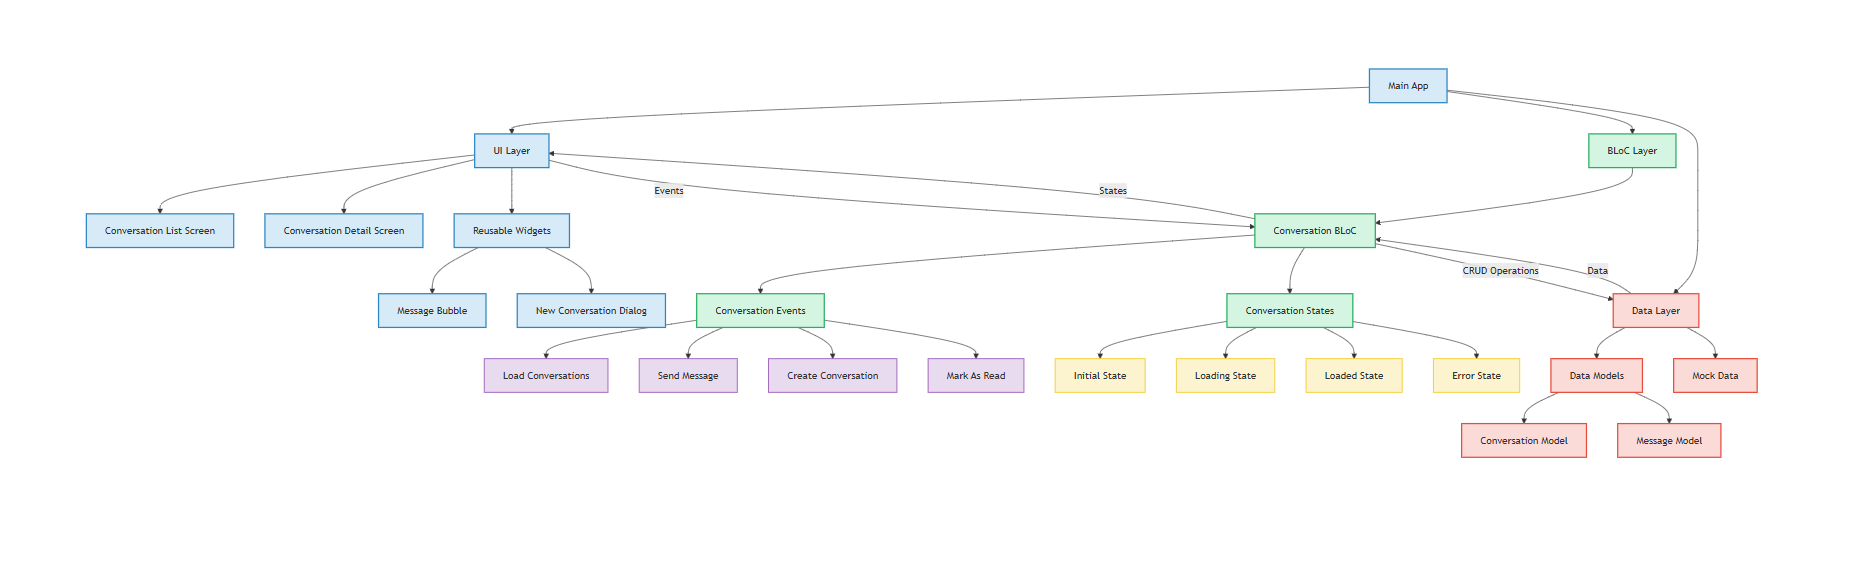
\includegraphics[width=0.9\textwidth]{../chat_app/screenshots/app_architecture_diagram.png}
    \caption{Diagramme illustrant l'architecture de l'application de chat.}
    \label{fig:app_architecture_diagram}
\end{figure}

Cette architecture favorise la testabilité (chaque couche peut être testée isolément), la maintenabilité (les modifications dans une couche ont un impact limité sur les autres) et la scalabilité de l'application.

\subsection{Le `ConversationBloc` et son Rôle Central}
% (La sous-section sur le BLoC a été renommée et déplacée ici pour un meilleur flux)
Le pattern BLoC (Business Logic Component) est le pilier de la gestion d'état. Notre `ConversationBloc` centralise la logique liée aux conversations et messages.

\begin{infobox}[title=Responsabilités du ConversationBloc]
\begin{itemize}
    \item \textbf{Chargement des données :} Initialiser et charger la liste des conversations.
    \item \textbf{Gestion des messages sortants :} Traiter l'envoi de messages, mettre à jour les données simulées et la conversation correspondante.
    \item \textbf{Simulation de la réception de messages :} Gérer l'arrivée simulée de messages.
    \item \textbf{Mise à jour de l'état global :} Émettre des états pour informer l'UI des changements.
    \item \textbf{Création de nouvelles conversations :} Gérer la logique de création d'une nouvelle instance de conversation.
\end{itemize}
\end{infobox}

Le `ConversationBloc` est injecté dans l'arborescence des widgets via `BlocProvider`, le rendant accessible aux écrans concernés.

\begin{lstlisting}[language=Dart, caption=Implémentation du ConversationBloc, style=dartstyle]
import 'package:flutter_bloc/flutter_bloc.dart';
import 'package:chat_app/bloc/conversation/conversation_event.dart';
import 'package:chat_app/bloc/conversation/conversation_state.dart';
import 'package:chat_app/models/conversation_model.dart';
import 'package:chat_app/models/message_model.dart';
import 'package:chat_app/data/mock_data.dart';

class ConversationBloc extends Bloc<ConversationEvent, ConversationState> {
  List<Conversation> _conversations = [];
  Map<String, List<Message>> _messages = {};

  ConversationBloc() : super(ConversationInitial()) {
    on<LoadConversations>(_onLoadConversations);
    on<SendMessage>(_onSendMessage);
    on<MarkConversationAsRead>(_onMarkConversationAsRead);
    on<CreateConversation>(_onCreateConversation);
  }

  void _onLoadConversations(LoadConversations event, Emitter<ConversationState> emit) {
    emit(ConversationLoading());
    // Charge les données simulées
    _conversations = List.from(mockConversations);
    _messages = Map.from(mockMessages);
    emit(ConversationLoaded(conversations: _conversations, messages: _messages));
  }

  void _onSendMessage(SendMessage event, Emitter<ConversationState> emit) {
    // Crée un nouveau message de l'utilisateur
    final newMessage = Message(
      id: DateTime.now().millisecondsSinceEpoch.toString(),
      conversationId: event.conversationId,
      content: event.text,
      isMe: true,
      timestamp: DateTime.now(),
    );

    // Crée une nouvelle map pour que Equatable détecte le changement
    final Map<String, List<Message>> updatedMessages = Map.from(_messages);
    updatedMessages[event.conversationId] = [...(updatedMessages[event.conversationId] ?? []), newMessage];
    _messages = updatedMessages;

    // Met à jour le dernier message et l'horodatage de la conversation
    final conversationIndex = _conversations.indexWhere((conv) => conv.id == event.conversationId);
    if (conversationIndex != -1) {
      final originalConversation = _conversations[conversationIndex];
      _conversations[conversationIndex] = Conversation(
        id: originalConversation.id,
        contactName: originalConversation.contactName,
        lastMessage: "You: ${event.text}", // Préfixe "You: " pour les messages de l'utilisateur
        timestamp: newMessage.timestamp,
        avatarUrl: originalConversation.avatarUrl, 
        unreadCount: 0, // Réinitialise le compteur de non-lus
      );
    }
    
    // Crée une nouvelle liste pour les conversations (important pour l'immutabilité)
    final List<Conversation> updatedConversationsList = List.from(_conversations);
    if (conversationIndex != -1) { 
        final updatedConversation = updatedConversationsList.removeAt(conversationIndex);
        updatedConversationsList.insert(0, updatedConversation); // Déplace la conversation en haut
    }
    _conversations = updatedConversationsList;

    // Émet l'état mis à jour avec le message de l'utilisateur
    emit(ConversationLoaded(conversations: updatedConversationsList, messages: updatedMessages));
    
    // Simulation d'une réponse automatique si activée
    if (event.autoReply) {
      // Simuler un délai avant la réponse du contact
      Future.delayed(const Duration(seconds: 1, milliseconds: 500), () {
        // Logique de réponse automatique...
      });
    }
  }
  
  // Autres méthodes pour gérer les événements...
}
\end{lstlisting}


\subsubsection{États (States) du `ConversationBloc`}
Les états décrivent l'état de l'application à un instant T. Ils sont immuables et héritent d'`Equatable`.
\begin{itemize}
    \item \textbf{`ConversationInitial`}: État par défaut avant toute opération.
    \item \textbf{`ConversationLoading`}: Indique un traitement de données en cours.
    \item \textbf{`ConversationLoaded`}: Les données sont chargées/mises à jour. Contient `conversations`, `activeConversationId`, et `activeMessages`.
    \item \textbf{`ConversationError`}: Une erreur est survenue. Contient un message d'erreur.
\end{itemize}

\begin{lstlisting}[language=Dart, caption=Définition des états du ConversationBloc (`conversation_state.dart`), style=dartstyle]
import 'package:equatable/equatable.dart';
import 'package:chat_app/models/conversation_model.dart';
import 'package:chat_app/models/message_model.dart';

abstract class ConversationState extends Equatable {
  const ConversationState();

  @override
  List<Object> get props => [];
}

class ConversationInitial extends ConversationState {}

class ConversationLoading extends ConversationState {}

class ConversationLoaded extends ConversationState {
  final List<Conversation> conversations;
  final Map<String, List<Message>> messages;

  const ConversationLoaded({required this.conversations, required this.messages});

  @override
  List<Object> get props => [conversations, messages];
}

class ConversationError extends ConversationState {
  final String message;

  const ConversationError({required this.message});

  @override
  List<Object> get props => [message];
}
\end{lstlisting}

\subsubsection{Événements (Events) du `ConversationBloc`}
Les événements sont des intentions envoyées au BLoC.
\begin{itemize}
    \item \textbf{`LoadConversations`}: Charge la liste initiale.
    \item \textbf{`CreateConversation`}: Crée une nouvelle conversation.
    \item \textbf{`SelectConversation`}: Sélectionne une conversation et charge ses messages.
    \item \textbf{`SendMessage`}: Envoie un message.
    \item \textbf{`SimulateReceiveMessage`}: Simule la réception d'un message.
\end{itemize}

\begin{lstlisting}[language=Dart, caption=Définition des événements du ConversationBloc (`conversation_event.dart`), style=dartstyle]
import 'package:equatable/equatable.dart';

abstract class ConversationEvent extends Equatable {
  const ConversationEvent();

  @override
  List<Object> get props => [];
}

class LoadConversations extends ConversationEvent {}

class SendMessage extends ConversationEvent {
  final String conversationId;
  final String text;
  final bool autoReply; // Add a parameter to control auto-reply

  const SendMessage({
    required this.conversationId,
    required this.text,
    this.autoReply = true, // Default to true
  });

  @override
  List<Object> get props => [conversationId, text, autoReply];
}

class MarkConversationAsRead extends ConversationEvent {
  final String conversationId;

  const MarkConversationAsRead({required this.conversationId});

  @override
  List<Object> get props => [conversationId];
}

class CreateConversation extends ConversationEvent {
  final String contactName;

  const CreateConversation({required this.contactName});

  @override
  List<Object> get props => [contactName];
}
\end{lstlisting}

\section{Modèles de Données}
Deux modèles principaux structurent les données : `Conversation` et `Message`. Ils utilisent `equatable` pour les comparaisons.

\subsection{Modèle `Conversation`}
Représente un fil de discussion.
\begin{itemize}
    \item `id` (String): Identifiant unique.
    \item `contactName` (String): Nom du contact.
    \item `lastMessage` (String): Aperçu du dernier message.
    \item `timestamp` (DateTime): Heure du dernier message.
    \item `avatarUrl` (String, optionnel): URL de l'avatar.
    \item `unreadCount` (int, optionnel): Nombre de messages non lus.
\end{itemize}

\begin{lstlisting}[language=Dart, caption=Modèle de données `Conversation` (`conversation_model.dart`), style=dartstyle]
import 'package:equatable/equatable.dart';

class Conversation extends Equatable {
  final String id;
  final String contactName;
  final String lastMessage;
  final DateTime timestamp;
  final String? avatarUrl;
  final int? unreadCount;

  const Conversation({
    required this.id,
    required this.contactName,
    required this.lastMessage,
    required this.timestamp,
    this.avatarUrl,
    this.unreadCount,
  });

  @override
  List<Object?> get props => [id, contactName, lastMessage, timestamp, avatarUrl, unreadCount];
}
\end{lstlisting}

\subsection{Modèle `Message`}
Représente un message individuel.
\begin{itemize}
    \item `id` (String): Identifiant unique du message.
    \item `conversationId` (String): ID de la conversation parente.
    \item `content` (String): Contenu textuel.
    \item `isMe` (bool): Vrai si envoyé par l'utilisateur actuel.
    \item `timestamp` (DateTime): Heure d'envoi.
\end{itemize}

\begin{lstlisting}[language=Dart, caption=Modèle de données `Message` (`message_model.dart`), style=dartstyle]
import 'package:equatable/equatable.dart';

class Message extends Equatable {
  final String id;
  final String conversationId;
  final String content;
  final bool isMe;
  final DateTime timestamp;

  const Message({
    required this.id,
    required this.conversationId,
    required this.content,
    required this.isMe,
    required this.timestamp,
  });

  @override
  List<Object?> get props => [id, conversationId, content, isMe, timestamp];
}
\end{lstlisting}

\begin{infobox}[title=Utilisation des Données Simulées (Mocks)]
Des listes `mockConversations` et `mockMessages` sont initialisées avec des données fictives. Le `ConversationBloc` interagit avec ces listes pour simuler les opérations de données, permettant un développement et des tests autonomes.
\end{infobox}


\section{Fonctionnalités Implémentées}
L'application s'articule autour de deux écrans principaux et d'un dialogue de création, fournissant les fonctionnalités essentielles d'une messagerie.

\subsection{Écran Liste des Conversations}
Point d'entrée de l'application (Figure \ref{fig:chats_list_screen}), cet écran offre un aperçu des discussions.
\begin{itemize}
    \item \textbf{Affichage de la liste :} Une `ListView.builder` affiche chaque conversation (avatar, nom, dernier message, timestamp). Un indicateur peut signaler si le dernier message est de l'utilisateur.
    \item \textbf{Badge de messages non lus :} Un badge numérique (visible pour "Charlie" et "Alice" sur la capture) indique les messages non lus.
    \item \textbf{Navigation :} Un appui sur une conversation ouvre sa vue détaillée.
    \item \textbf{Création de conversation :} Un `FloatingActionButton` (+) ouvre un dialogue modal (Figure \ref{fig:new_conversation_dialog_screen}) pour entrer le nom d'un nouveau contact.
\end{itemize}

\begin{figure}[htbp]
    \centering
    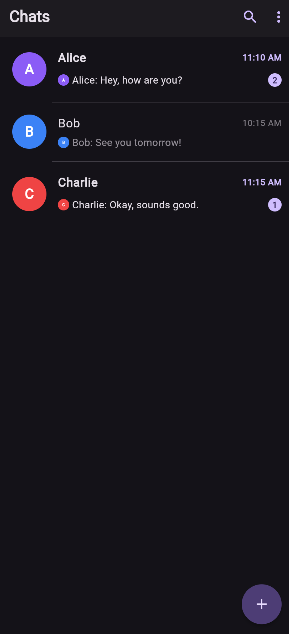
\includegraphics[height=0.6\textheight, keepaspectratio]{../chat_app/screenshots/chats_list_screen.png} 
    \caption{Capture d'écran de la liste des conversations ("Chats").}
    \label{fig:chats_list_screen}
\end{figure}

\begin{figure}[htbp]
    \centering
    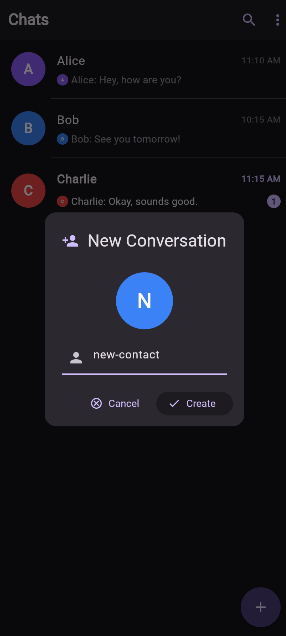
\includegraphics[height=0.6\textheight, keepaspectratio]{../chat_app/screenshots/new_conversation_dialog_screen.png} 
    \caption{Dialogue modal "New Conversation" pour la création d'un nouveau contact.}
    \label{fig:new_conversation_dialog_screen}
\end{figure}


\subsection{Écran de la Conversation Détaillée}
Cet écran est le lieu de l'interaction de chat.
\begin{itemize}
    \item \textbf{Affichage des messages :} Une `ListView` (avec `reverse: true`) affiche les messages sous forme de bulles, les plus récents en bas.
    \item \textbf{Informations du contact :} L'`AppBar` montre l'avatar, le nom (ex: "Alice") et le statut ("Online"). Des icônes d'appel et de menu sont présentes.
    \item \textbf{Séparateurs temporels :} Des indicateurs comme "Today, 11:05 AM" structurent la chronologie des messages.
    \item \textbf{Champ de saisie :} Un `TextField` ("Type a message...") et un bouton d'envoi permettent de composer des messages. L'icône "trombone" suggère l'ajout de pièces jointes.
    \item \textbf{Différenciation visuelle :} Les messages de l'utilisateur (droite, fond violet clair, statut par double coche) sont distincts de ceux du contact (gauche, fond gris foncé).
\end{itemize}

\begin{lstlisting}[language=Dart, caption=Implémentation des bulles de messages, style=dartstyle]
Widget _buildMessageBubble(Message message) {
  final theme = Theme.of(context);
  final isMe = message.isMe;
  
  return Padding(
    padding: EdgeInsets.only(
      bottom: 12,
      left: isMe ? 64 : 8,
      right: isMe ? 8 : 64,
    ),
    child: Row(
      mainAxisAlignment: isMe ? MainAxisAlignment.end : MainAxisAlignment.start,
      crossAxisAlignment: CrossAxisAlignment.end,
      children: [
        // Afficher l'avatar pour les messages reçus
        if (!isMe) ...[
          BlocBuilder<ConversationBloc, ConversationState>(
            builder: (context, state) {
              if (state is ConversationLoaded) {
                final conversation = state.conversations.firstWhere(
                  (conv) => conv.id == widget.conversationId,
                  orElse: () => Conversation(id: '', contactName: 'Chat', lastMessage: '', timestamp: DateTime.now()),
                );
                return AvatarUtils.getAvatar(
                  name: conversation.contactName,
                  radius: 16,
                );
              }
              return const SizedBox(width: 32, height: 32); // Placeholder
            },
          ),
          const SizedBox(width: 8),
        ],
        
        // Bulle de message
        Flexible(
          child: Container(
            constraints: BoxConstraints(
              maxWidth: MediaQuery.of(context).size.width * 0.75,
            ),
            padding: const EdgeInsets.symmetric(horizontal: 16, vertical: 10),
            decoration: BoxDecoration(
              color: isMe ? theme.colorScheme.primary : theme.colorScheme.surface,
              borderRadius: BorderRadius.only(
                topLeft: const Radius.circular(16),
                topRight: const Radius.circular(16),
                bottomLeft: isMe ? const Radius.circular(16) : const Radius.circular(4),
                bottomRight: isMe ? const Radius.circular(4) : const Radius.circular(16),
              ),
              boxShadow: [
                BoxShadow(
                  color: Colors.black.withOpacity(0.05),
                  blurRadius: 4,
                  offset: const Offset(0, 2),
                ),
              ],
            ),
            child: Column(
              crossAxisAlignment: CrossAxisAlignment.start,
              children: [
                Text(
                  message.content,
                  style: TextStyle(
                    color: isMe ? theme.colorScheme.onPrimary : theme.colorScheme.onSurface,
                    fontSize: 16,
                  ),
                ),
                const SizedBox(height: 4),
                Row(
                  mainAxisSize: MainAxisSize.min,
                  mainAxisAlignment: MainAxisAlignment.end,
                  children: [
                    Text(
                      DateFormat('h:mm a').format(message.timestamp),
                      style: TextStyle(
                        fontSize: 12,
                        color: isMe ? theme.colorScheme.onPrimary.withOpacity(0.7) : theme.colorScheme.onSurface.withOpacity(0.6),
                      ),
                    ),
                    if (isMe)
                      Padding(
                        padding: const EdgeInsets.only(left: 4),
                        child: Icon(
                          Icons.done_all,
                          size: 14,
                          color: theme.colorScheme.onPrimary.withOpacity(0.7),
                        ),
                      ),
                  ],
                ),
              ],
            ),
          ),
        ),
        // Espace pour l'avatar des messages envoyés
        if (isMe) const SizedBox(width: 32),
      ],
    ),
  );
}
\end{lstlisting}


La figure \ref{fig:chat_detail_alice_screen} montre une conversation existante avec "Alice".

\begin{figure}[htbp]
    \centering
    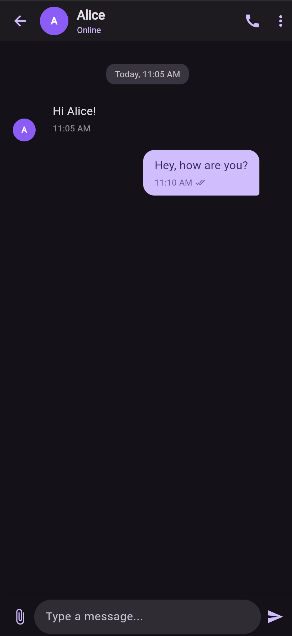
\includegraphics[height=0.6\textheight, keepaspectratio]{../chat_app/screenshots/chat_detail_alice_screen.png} 
    \caption{Vue détaillée d'une conversation existante avec "Alice".}
    \label{fig:chat_detail_alice_screen}
\end{figure}

Pour une nouvelle conversation avec "new-contact" (créée via le dialogue de la Figure \ref{fig:new_conversation_dialog_screen}), l'écran est initialement vide (Figure \ref{fig:new_conversation_empty_screen}), avec une incitation à démarrer la discussion.

\begin{figure}[htbp]
    \centering
    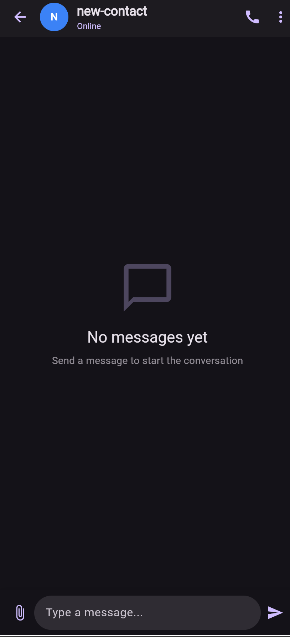
\includegraphics[height=0.6\textheight, keepaspectratio]{../chat_app/screenshots/new_conversation_empty_screen.png}
    \caption{Nouvelle conversation avec "new-contact", initialement vide.}
    \label{fig:new_conversation_empty_screen}
\end{figure}

Après l'envoi du premier message, par exemple "Welcome to my app", il s'affiche (Figure \ref{fig:new_conversation_first_message_screen}).

\begin{figure}[htbp]
    \centering
    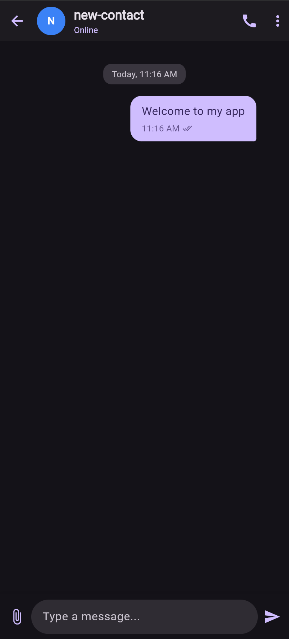
\includegraphics[height=0.6\textheight, keepaspectratio]{../chat_app/screenshots/new_conversation_first_message_screen.png}
    \caption{Nouvelle conversation avec "new-contact" après l'envoi du premier message.}
    \label{fig:new_conversation_first_message_screen}
\end{figure}


\section{Navigation entre les Écrans}
La navigation est assurée par le widget `Navigator` de Flutter, utilisant des `MaterialPageRoute`.
\begin{itemize}
    \item \textbf{De la Liste à la Détail Conversation :} Lors de la sélection d'une conversation, `Navigator.push()` est appelé, passant l'`id` de la conversation. L'événement `SelectConversation` du BLoC est déclenché en amont pour charger les messages correspondants.
    \begin{lstlisting}[language=Dart, caption=Navigation vers l'écran de détail, style=dartstyle]
// Dans ConversationListScreen, onTap d'un ListTile:
onTap: () {
  context.read<ConversationBloc>().add(MarkConversationAsRead(conversationId: conversation.id));
  Navigator.push(
    context,
    MaterialPageRoute(
      builder: (_) => BlocProvider.value(
        value: BlocProvider.of<ConversationBloc>(context),
        child: ConversationDetailScreen(conversationId: conversation.id),
      ),
    ),
  );
}
\end{lstlisting}
    \item \textbf{Création d'une Nouvelle Conversation :} Le `FloatingActionButton` de la liste des conversations ouvre un dialogue (Figure \ref{fig:new_conversation_dialog_screen}). Après saisie du nom et confirmation, un événement `CreateConversation` est envoyé au BLoC. Si la création réussit, l'application navigue vers l'écran `ConversationDetailScreen` pour cette nouvelle conversation (initialement vide, voir Figure \ref{fig:new_conversation_empty_screen}).

\begin{lstlisting}[language=Dart, caption=Dialogue de création d'une nouvelle conversation, style=dartstyle]
void _showCreateConversationDialog(BuildContext parentContext) {
  final theme = Theme.of(parentContext);
  final TextEditingController nameController = TextEditingController();
  String previewName = '';
  
  showDialog(
    context: parentContext,
    builder: (BuildContext dialogContext) {
      return StatefulBuilder(
        builder: (context, setState) {
          return AlertDialog(
            title: Row(
              children: [
                Icon(Icons.person_add, color: theme.colorScheme.primary),
                const SizedBox(width: 12),
                const Text('New Conversation'),
              ],
            ),
            content: Column(
              mainAxisSize: MainAxisSize.min,
              children: [
                if (previewName.isNotEmpty) ...[
                  const SizedBox(height: 8),
                  AvatarUtils.getAvatar(
                    name: previewName,
                    radius: 40,
                  ),
                  const SizedBox(height: 16),
                ],
                TextField(
                  controller: nameController,
                  decoration: const InputDecoration(
                    hintText: "Enter contact's name",
                    prefixIcon: Icon(Icons.person),
                  ),
                  autofocus: true,
                  textCapitalization: TextCapitalization.words,
                  onChanged: (value) {
                    setState(() {
                      previewName = value;
                    });
                  },
                ),
              ],
            ),
            actions: <Widget>[
              TextButton.icon(
                icon: const Icon(Icons.cancel_outlined),
                label: const Text('Cancel'),
                onPressed: () {
                  Navigator.of(dialogContext).pop();
                },
              ),
              ElevatedButton.icon(
                icon: const Icon(Icons.check),
                label: const Text('Create'),
                onPressed: () {
                  if (nameController.text.trim().isNotEmpty) {
                    parentContext.read<ConversationBloc>().add(
                      CreateConversation(contactName: nameController.text.trim())
                    );
                    Navigator.of(dialogContext).pop();
                  }
                },
              ),
            ],
          );
        }
      );
    },
  );
}
\end{lstlisting}

    \item \textbf{Retour :} Le bouton "retour" de l'`AppBar` ou le geste de retour système utilisent `Navigator.pop(context)` pour revenir à l'écran précédent. La liste des conversations est mise à jour par le BLoC pour refléter les éventuels changements.
\end{itemize}

\begin{infobox}[title=Gestion des Routes et Accès au BLoC]
Le `ConversationBloc` est fourni une seule fois en haut de l'arborescence des widgets via `BlocProvider`. Il est ensuite accessible dans les écrans descendants via `context.read<ConversationBloc>()` pour déclencher des événements ou `BlocBuilder` / `context.watch<ConversationBloc>()` pour réagir aux changements d'état. Pour des applications plus complexes, l'utilisation de routes nommées ou d'un `RouterDelegate` est préférable pour une meilleure organisation.
\end{infobox}

\section{Code Source}
Le code source complet de cette application Flutter est hébergé sur GitHub et accessible publiquement :
\begin{center}
    \url{https://github.com/youssef-faik/chat_app} % ASSUREZ-VOUS QUE CETTE URL EST CORRECTE
\end{center}
\begin{warningbox}[title=Accès et Structure du Dépôt]
Il est impératif que le dépôt GitHub soit public ou que les évaluateurs disposent des droits d'accès nécessaires. Une structure de projet claire, respectant les conventions Flutter (par exemple, séparation des répertoires `blocs`, `models`, `ui`/`widgets`, `screens`/`pages`), est fortement recommandée pour faciliter la compréhension et l'évaluation du code.
\end{warningbox}

\section{Conclusion et Perspectives}
Ce projet a permis de développer une application de chat fonctionnelle en utilisant Flutter et le pattern BLoC, atteignant ainsi les objectifs fixés. L'architecture mise en place favorise la maintenabilité et l'évolutivité. Les fonctionnalités de base, telles que la liste des conversations, la vue détaillée des messages, et la création de nouvelles discussions, ont été implémentées avec succès à l'aide de données simulées.

Ce travail constitue une fondation solide pour des développements futurs. Parmi les perspectives d'évolution, on peut citer :
\begin{itemize}
    \item \textbf{Intégration d'un Backend Réel :} Remplacer les données simulées par une connexion à une base de données distante (ex: Firebase, Supabase) et un service de messagerie en temps réel (WebSockets).
    \item \textbf{Authentification des Utilisateurs :} Mettre en place un système de connexion et d'inscription.
    \item \textbf{Notifications Push :} Intégrer des notifications pour alerter les utilisateurs de nouveaux messages.
    \item \textbf{Fonctionnalités de Chat Avancées :} Ajouter des indicateurs de frappe, statuts des messages (envoyé, délivré, lu), partage de médias, messages vocaux.
    \item \textbf{Tests Approfondis :} Écrire des tests unitaires pour les BLoCs, des tests de widgets pour l'UI, et des tests d'intégration.
    \item \textbf{Optimisation et UI/UX :} Améliorer les performances, peaufiner l'interface utilisateur avec des animations et des thèmes personnalisables.
\end{itemize}
En conclusion, ce projet démontre la puissance de Flutter et BLoC pour construire des applications mobiles modernes et robustes.

\end{document}